\documentclass[letterpaper,10pt,titlepage]{article}

\usepackage{graphicx}                                        
\usepackage{amssymb}                                         
\usepackage{amsmath}                                         
\usepackage{amsthm} 
\usepackage{verbatim}                                         

\usepackage{alltt}                                           
\usepackage{float}
\usepackage{color}
\usepackage{url}
\usepackage{fancybox}
\usepackage{verbatim}

\usepackage{balance}
\usepackage[TABBOTCAP, tight]{subfigure}
\usepackage{enumitem}
\usepackage{pstricks, pst-node}
\usepackage{texments}

\usepackage{geometry}
\geometry{textheight=9in, textwidth=6.5in}

\newcommand{\cred}[1]{{\color{red}#1}}
\newcommand{\cblue}[1]{{\color{blue}#1}}
\newcommand{\tab}{\hspace*{2em}}

\usepackage{hyperref}
\usepackage{geometry}

\def\name{Eric Timmerman, Stephanie Ison, Geoffrey Corey}

%% The following metadata will show up in the PDF properties
\hypersetup{
  colorlinks = true,
  urlcolor = black,
  pdfauthor = {\name},
  pdfkeywords = {cs325 ``algorithmic analysis''},
  pdftitle = {CS 325: Project 4},
  pdfsubject = {CS 325: Project 4},
  pdfpagemode = UseNone
}

\begin{document}
\hfill \name

\hfill \today

\hfill CS 325 Proj 4

\section{Warm-Up Question}
\subsection*{General Problem}
min $t$\\
$a*x_{i} + b - y_{i} >= t$\\
$-a*x{i} - b + y_{i} >= t$\\
where $x_{i}$ and $y_{i}$ are from the set of data, finding $a$ and $b$
\subsection*{Specific Problem}
$a = 1$\\
$b = -0.857$

\subsection*{Plot}
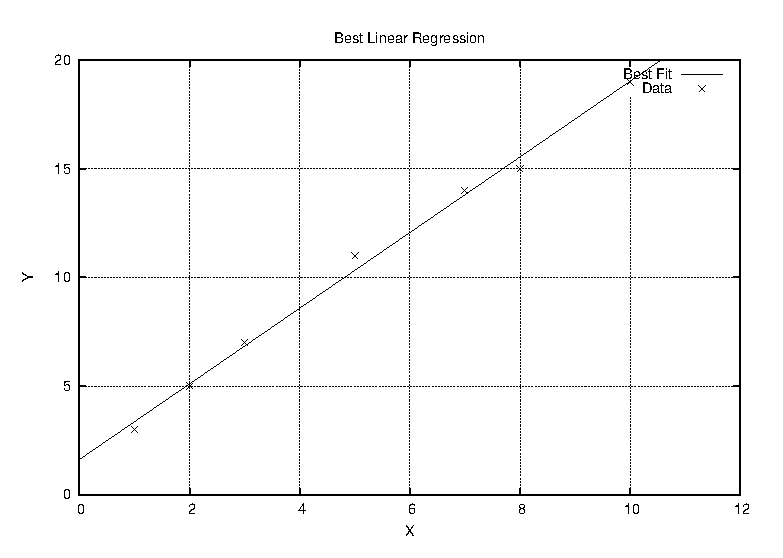
\includegraphics[width=\textwidth]{warmup.eps}

\section{Warming-Up Question}
\subsection*{Linear Program Description}
\subsection*{X Constants}
\subsection*{Plot}
\subsection*{$X_{1}$ Century Trend}

\end{document}
